\subsection{Solar Neutrinos - GDOG, R Bonventre}
%\paragraph{Motivation}
%BRIEF intro to physics motivation, and status of the field: our major competitors
%\paragraph{XX with THEIA}
%What we bring to the table - pros of THEIA design \newline
%Sensitivity estimates with baseline design (one of THEIA i--iii)
%\paragraph{Detector Requirements}
%A summary of the impact of different detector choices i.e. what happens if we stray from the relevant baseline


Both water Cherenkov and liquid scintillator detectors have a long history of successful observation of solar neutrinos.  A number of open questions remain, including: first detection of neutrinos from the sub-dominant CNO fusion cycle, as a method to resolve the solar metallicity; a precision probe of the transition region between low-energy vacuum-dominated oscillation, below 1~MeV, and matter-dominated regime above 5~MeV, as a sensitive search for new physics effects; tests of solar luminosity through precision measurements of pep and pp neutrinos; tests of the solar temperature and, potentially, separation of the different components of the CNO flux to probe the extent to which this cycle is in equilibrium in the Sun's core.

Many of these questions can be addressed by \textsc{Theia}'s combination of a low-threshold directional detector, along with the potential for isotope loading.  \textsc{Theia} would provide unprecedented sensitivity to solar neutrinos via two channels:
\begin{enumerate}
\item {\it Huge statistics for elastic scattering (ES) events at low energy}.  
The LENA collaboration~\cite{lena} have explored in detail the power of a large-scale scintillator detector for resolving open questions in solar neutrino physics, such as determining the solar metallicity via a measurement of neutrinos from the sub-dominant CNO fusion cycle.  \textsc{Theia} would have similar capability, along with the additional advantage of being able to distinguish ES events from backgrounds (such as $^{210}$Bi) using directionality.

\item {\it Potential charged-current (CC) detection via isotope loading e.g. $^7$Li}~\cite{li}.  
The differential CC cross section for neutrino interaction on $^7$Li is extremely sharply peaked.  As a result, CC neutrino detection provides a high-precision measurement of the incoming neutrino energy, allowing extraction of the low-energy $^8$B spectrum. This would provide a sensitive search for new physics via a probe of the transition region in the neutrino spectrum between vacuum-dominated and matter-enhanced oscillations.  There is also the potential to separate the different components of the CNO flux via a shape analysis.

\end{enumerate}

\subsubsection{ES Measurements}
The sensitivity to CNO and pep solar neutrinos of an unloaded WbLS detector via the ES interaction has been studied in ~\cite{richiegdog}.  

By performing a two-dimensional  binned maximum likelihood fit  in energy and direction relative to the Sun, $\cos\theta_{\odot}$, neutrino fluxes are separated from each other, as well as  from certain sources of radioactive background.  
For each signal the $\cos\theta_{\odot}$ distribution was determined fully analytically.
All non-neutrino signals were assumed to be flat. For the solar signals the
electron direction relative to the Sun was determined
based on the differential cross sections. This was then convolved with a chosen angular resolution.  The energy response was determined semi-analytically, based on chosen detector parameters such as target light yield and photocathode coverage.  
This paper summarises the assumptions made regarding detector configuration and performance, and the resulting sensitivity to solar neutrinos. Full details of the analysis are described in~\cite{richiegdog}.  

The baseline detector configuration was chosen to be a 50-kT detector with 90\% PMT coverage, a 5\% WbLS target, and $25^\circ$ angular resolution, with baseline background levels as given in Table \ref{t:bg}. The dominant cosmogenic background, from \isotope[11]{C}, was conservatively taken to be at the Borexino level, scaled by the respective target mass.  If located at the proposed site at LBNF this background would in fact be significantly lower. All results assume a five year livetime.

\begin{table}
  {  \begin{tabular}{c c c c c}
    & H2O Level (g/gH2O) & LS Level (g/gLAB)\\
    \hline
    \isotope[238]{U} Chain & 6.63e-15 \cite{SNObg} & 1.6e-17 \cite{Borbg1}\\
    \isotope[232]{Th} Chain & 8.8e-16 \cite{SNObg} & 6.8e-18 \cite{Borbg1}\\
    \isotope[40]{K} & 6.1e-16$^a$ & 1.3e-18 \cite{Borbg2}\\
    \isotope[85]{Kr} & 2.4e-25$^b$ & 2.4e-25 \cite{Borbg2} \\
    \isotope[39]{Ar} & 2.75e-24$^b$ & 2.75e-24 \cite{Borbg2} \\
    \isotope[210]{Bi} & 3.78e-28$^b$ & 3.78e-28 \cite{Borbg2} \\
    \isotope[11]{C} & 0 & 1.0e5 (ev/kT/year) \cite{bor_be7} \\
  \end{tabular}
}
  \caption{Background assumptions for the baseline configuration. \\
  $^a$ The \isotope[40]{K} level in water is taken to be 0.1x the Borexino measurement \cite{borex_ctf}\\
  $^b$ The \isotope[85]{Kr}, \isotope[39]{Ar}, and \isotope[210]{Bi} levels in water are taken to be the Borexino measured level in scintillator \cite{Borbg2}, although levels increased by several orders of magnitude are explored \label{t:bg}
}
\end{table}

The impact of each choice of detector configuration and background level was  studied, including the target mass, the percentage loading of LS in the WbLS target, photocathode coverage, angular resolution, and background levels.  Energy reconstruction was performed semi-analytically, and the resolution was determined from a combination of the target light yield and photocathode coverage.  The effect of systematic uncertainties in both energy scale and resolution were considered.  A full reconstruction of event direction was not attempted; rather, the impact of certain values of angular resolution was considered.  In practice, the achievable angular resolution would be correlated with other detector parameters, such as the percent LS loading -- a higher fractional loading makes separation of the prompt Cherenkov signal from the isotropic scintillation more challenging, thus limiting the angular resolution.  This separation could be further enhanced by deploying fast photon sensors, such as LAPPDs~\cite{mcp--lappd3}.

The fit uncertainty for each signal with the baseline detector configuration and background assumptions is shown in Table \ref{tab:tenthk40detail}.

\begin{table}
  {  \begin{tabular}{c c c c c}
    Signal & Normalization sensitivity (\%) \\
    \hline
    \isotope[8]{B} $\nu$ & 0.4 \\
    \isotope[7]{Be} $\nu$ & 0.4 \\
    pep $\nu$ & 3.8 \\
    CNO $\nu$ & 5.3 \\
    \isotope[210]{Bi} & 0.1 \\
    \isotope[11]{C} & 11.5 \\
    \isotope[85]{Kr} & 10.5 \\
    \isotope[40]{K} & 0.04 \\
    \isotope[39]{Ar}/\isotope[210]{Po} & 21.9 \\
    \isotope[238]{U} chain & 0.02 \\
    \isotope[232]{Th} chain & 0.05 \\
  \end{tabular}}
\caption{Fit uncertainty for 5 years of data with the baseline configuration and background assumptions }
  \label{tab:tenthk40detail}
\end{table}

The impact on the CNO solar neutrino sensitivity  of detector size, LS fraction, and angular resolution for the baseline background assumptions is shown in Table \ref{tab:tenthk40} and Fig.~\ref{fig:fitresults}.

\begin{table}
 { \begin{tabular}{c c | c c c c}
      Target mass & WbLS & \multicolumn{4}{l}{Angular resolution} \\
             & & $25^\circ$ & $35^\circ$ & $45^\circ$ & $55^\circ$\\
             \hline
             50 kT & 0.5\% & 6.2 & 8.8 & 11.2 & 13.5 \\
             50 kT & 1\% & 6.1 & 8.7 & 11.0 & 13.4 \\
             50 kT & 2\% & 6.2 & 8.9 & 11.4 & 13.8 \\
             50 kT & 3\% & 5.9 & 8.4 & 10.7 & 13.0 \\
             50 kT & 4\% & 5.5 & 7.9 & 10.1 & 12.3 \\
             50 kT & 5\% & 5.3 & 7.6 & 9.7 & 11.8 \\
             \hline
             25 kT & 0.5\% & 8.5 & 12.2 & 15.6 & 18.7 \\
             25 kT & 1\% & 8.5 & 12.1 & 15.0 & 18.4 \\
             25 kT & 2\% & 8.5 & 12.1 & 15.5 & 18.7 \\
             25 kT & 3\% & 8.0 & 11.5 & 14.6 & 17.7 \\
             25 kT & 4\% & 7.6 & 10.9 & 13.9 & 16.8 \\
             25 kT & 5\% & 7.3 & 10.5 & 13.3 & 16.2 \\
  \end{tabular}}
  \caption{CNO flux sensitivity (\%) as a function of target mass, WbLS \% and angular resolution for 5 years of data with 90\% PMT coverage and the baseline background assumptions }
\label{tab:tenthk40}
\end{table}

\begin{figure}
  \includegraphics[width=3.5in]{solar/{borex01k_cno}.pdf}
  \caption{CNO sensitivity as a function of scintillator fraction and angular resolution for a 50 kT detector after 5 years of running with the baseline background assumptions \label{fig:fitresults}}
\end{figure}

A study of both energy scale and resolution systematics shows that these can be constrained by the data to sub-percent levels, making them sub-dominant in the final flux sensitivities. 

The sensitivity was shown to be extremely robust to background level variations of several orders of magnitude at the baseline angular resolution, and to the assumed level of $\beta -- \alpha$ discrimination and BiPo coincidence  rejection.  Even the dominant background to the Borexino measurement, \isotope[11]{C}, was shown to have a small impact, demonstrating that the depth of the experiment site is not a critical factor.  This is to be expected, since the directional resolution provides extremely strong separation between solar neutrino signal events and the uniform background events.  The level of $^{40}$K was observed to have the largest impact: an increase of x10 in this background reduces the CNO sensitivity by a factor of 2.  
$^{40}$K is a dominant background at
low energies. This is due to the much higher contamination in the water component of the WbLS compared to the relatively cleaner scintillator -- even assuming an order of magnitude improvement over the level measured in water by Borexino and SNO. The $^{40}$K
background in water was not critical for these previous measurements, and so it may be
possible to further reduce the level with additional effort. The SNO water
processing plant could be improved by increasing the frequency of replacing ion
exchange columns or by distilling the water. A successful measurement in WbLS would rely on such improvements.

\subsubsection{CC Measurements}

The potential for CC measurements in Theia was studied in ~\cite{asdc}.  That work is summarised here.

Several factors contribute to the choice of isotope for loading into a scintillator detector.  $^{37}$Cl and $^{71}$Ga have been used successfully by radiochemical experiments from the late 1960s to the present day.  $^{7}$Li has been considered as a favorable alternative~\cite{rcli} but such a detector was never constructed.  $^{7}$Li was also proposed as an additive to a water detector in~\cite{li}; such a detector would have excellent sensitivity to the high end of the $^8$B spectrum, but would be limited in threshold. 
As seen in Fig.~\ref{f:clga}, $^{71}$Ga and $^{7}$Li both have more favorable cross sections than $^{37}$Cl, particularly at low energies.    However, the cost of $^{71}$Ga would likely be prohibitive in a liquid scintillator experiment.  The relatively large differential uncertainties on the $^{71}$Ga cross section would also smear out any extracted spectrum whereas the cross sections on $^{37}$Cl and $^{7}$Li are known to extremely high precision.  The $^{37}$Cl cross section has been mapped using the $\beta$ decay of $^{37}$Ca.  
The CC interaction of $\nu_e$ on $^{7}$Li is shown in Eq.~(\ref{e:li}).
\begin{equation}\label{e:li}
^{7}Li + \nu_e \rightarrow\, ^{7}Be + e^- \quad \rm{(Q = 862~keV)}
\end{equation}
$^{7}$Li has only two significant transitions: a mixed Fermi and Gamow-Teller transition to the ground state of $^{7}$Be with a threshold of 0.862~MeV; and a super-allowed Gamow-Teller transition to the first excited state at $\sim$430~keV, which decays with a lifetime of $\tau \sim$200~fs.   The scattering is very hard, transferring almost all incident energy to the scattered electron.  If one could differentiate between the electron of the ground state and the $e^- + \gamma$ of the first excited state one would have a high-precision reconstruction of neutrino energy.  The two states also have precisely known angular distributions, which could then be used as an additional handle to differentiate signal from background.  Even without the use of particle ID to differentiate between states the contribution of the two is known precisely from theory, so the difference in threshold can be used to demonstrate that the two are being seen in the correct proportions.
There is also the potential to observe NC interactions on $^{7}$Li (Fig.~\ref{f:clga}), exciting the analog 478~keV first excited state of $^{7}$Li, which then decays with a lifetime of $\tau \sim$105~fs.  On preliminary investigation $^{7}$Li would thus appear to be the preferred isotope.  However, other factors may be important, such as the effect of isotope loading on scintillator optics.

\begin{figure}[!ht]
\begin{center}
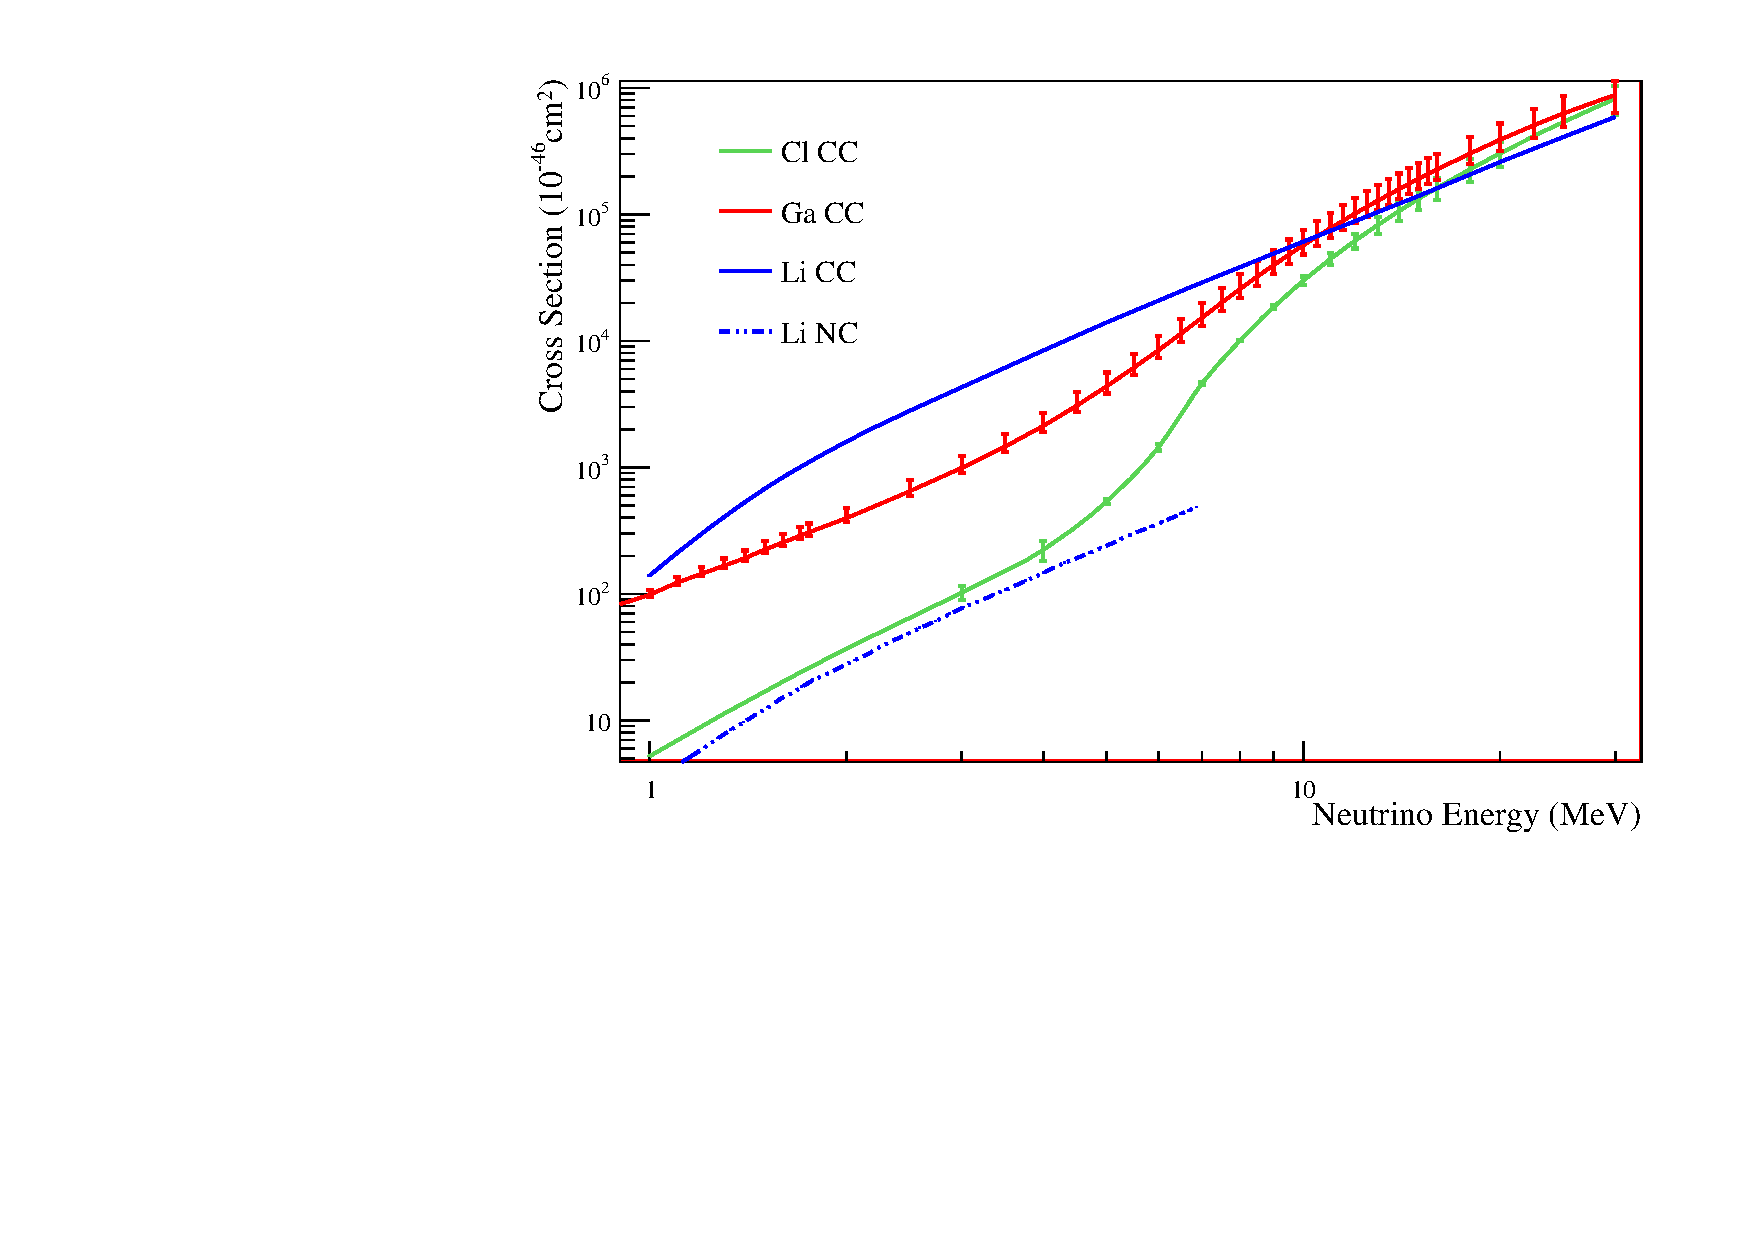
\includegraphics[width=3.5in]{solar/xsecnc.pdf}
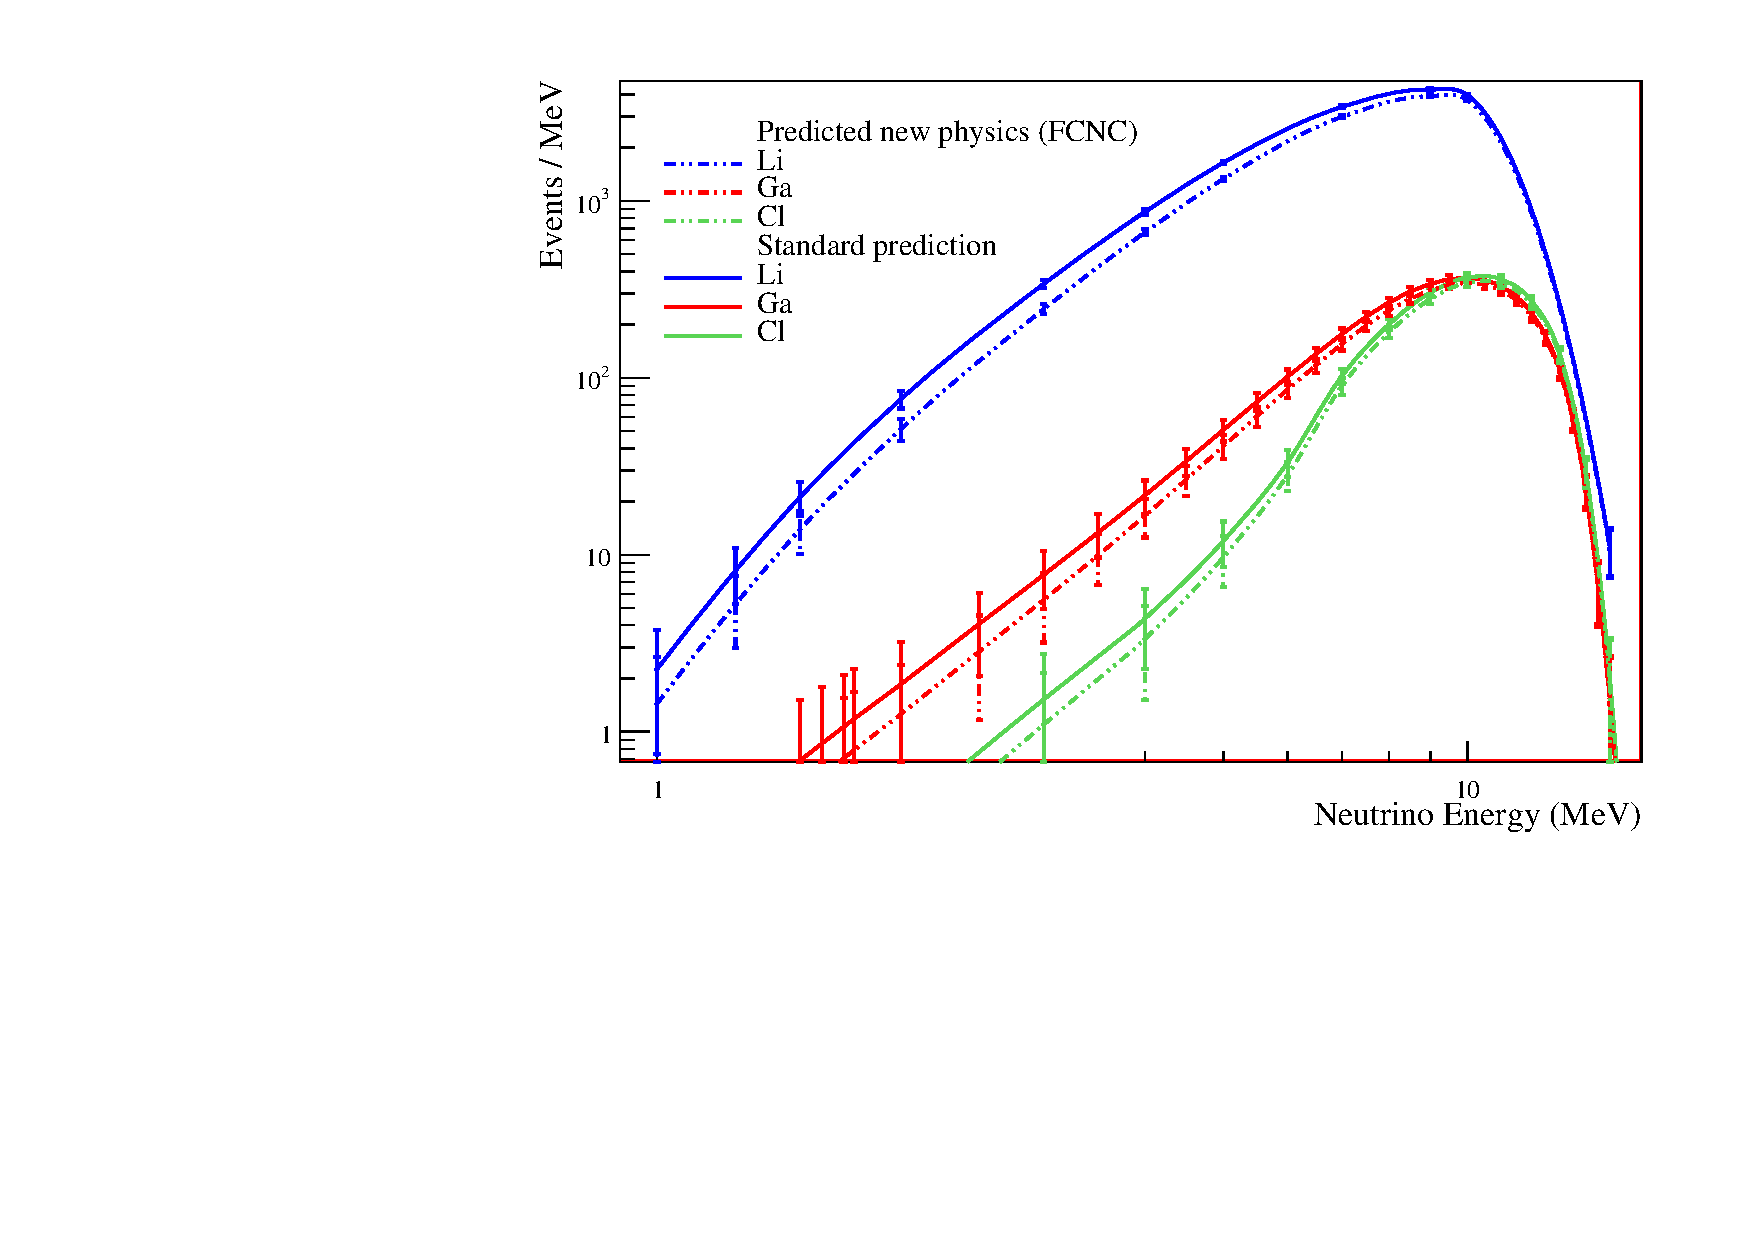
\includegraphics[width=3.5in]{solar/spectrume.pdf}
\caption{(Top) The cross section for CC neutrino interaction on $^{37}$Cl (green), $^{71}$Ga (red), and $^{7}$Li (blue) targets and NC on $^{7}$Li (blue dashed).  Data taken from~\cite{sigcl},~\cite{sigga},~\cite{sigli}, and~\cite{signc}, respectively. Although the differential uncertainties are not shown, the uncertainty on the lithium cross section is roughly 1\%~\cite{li}. (Bottom)  Predicted solar neutrino event spectra for 5 years of data-taking, with 1\% loading by mass of candidate isotopes in a 30-kT WbLS-filled ASDC detector. Solid lines show the standard solar neutrino oscillation prediction.  Dashed lines are for a flat neutrino spectrum to low energies, indicative of new physics interactions.  $^7$Li is the most favorable choice due to a high cross section for neutrino absorption.  Five years of data taking results in over 17~$\sigma$ separation in the integral flux, and correspondingly high precision (several $\sigma$ significance) on the extracted spectrum.
\label{f:clga}}
\end{center}
\vspace{-1.\baselineskip}
\end{figure}

Figure~\ref{f:solarspec} shows the predicted spectrum for the \textsc{Theia} detector assuming a 30-kT fiducial volume loaded with 1\% $^7$Li by mass, and a conservative light yield of 100 photoelectrons per MeV.  Standard MSW oscillation is assumed.  Solid lines show the CC interactions and dashed lines show ES detection.  The ES statistics by far outweigh the CC (as expected at a low \%-level loading); however, the use of directionality would allow excellent separation.  The right-hand panel shows the spectrum with a cut placed on $\cos\theta_{\odot}=0.4$ (where $\theta_{\odot}$ is the angle between the event direction and a vector pointing back to the Sun), which reduces the ES signals by more than 2 orders of magnitude.  (Angular resolution equivalent to SK-III was assumed).  In practice a more sophisticated analysis would link the normalization of the ES and CC neutrino signals via their known cross sections, allowing the ES to be used to separate events from radioactive and cosmogenic backgrounds such as $^{210}$Bi and $^{11}$C, and the CC to provide the spectral sensitivity.  The power of the CC signal can be observed in particular in the $^8$B spectrum, which has a distinctive shape, and the strong peak in the $pep$ signal in comparison to the broad ES spectrum.


\begin{figure}[!ht]
\begin{center}
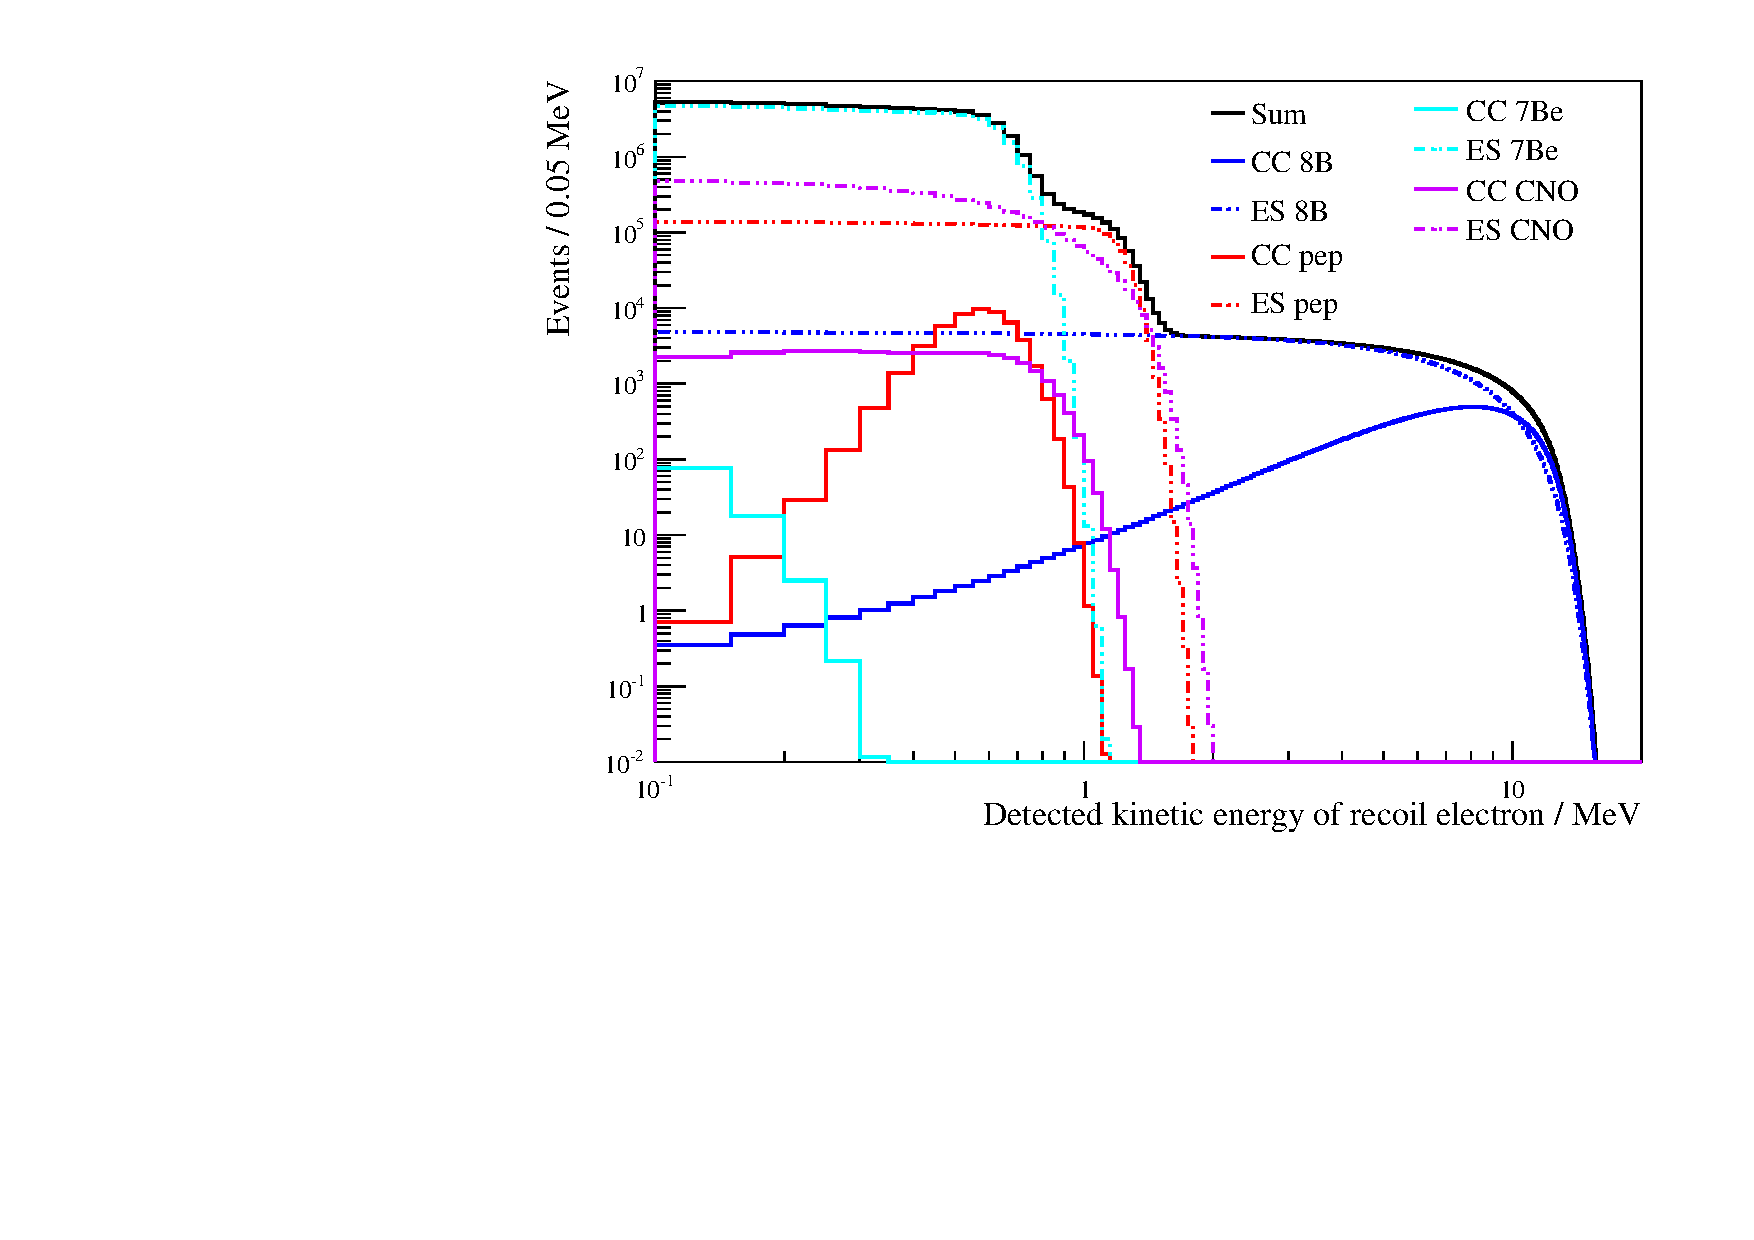
\includegraphics[width=3.5in]{solar/TotalSpectrum.pdf}
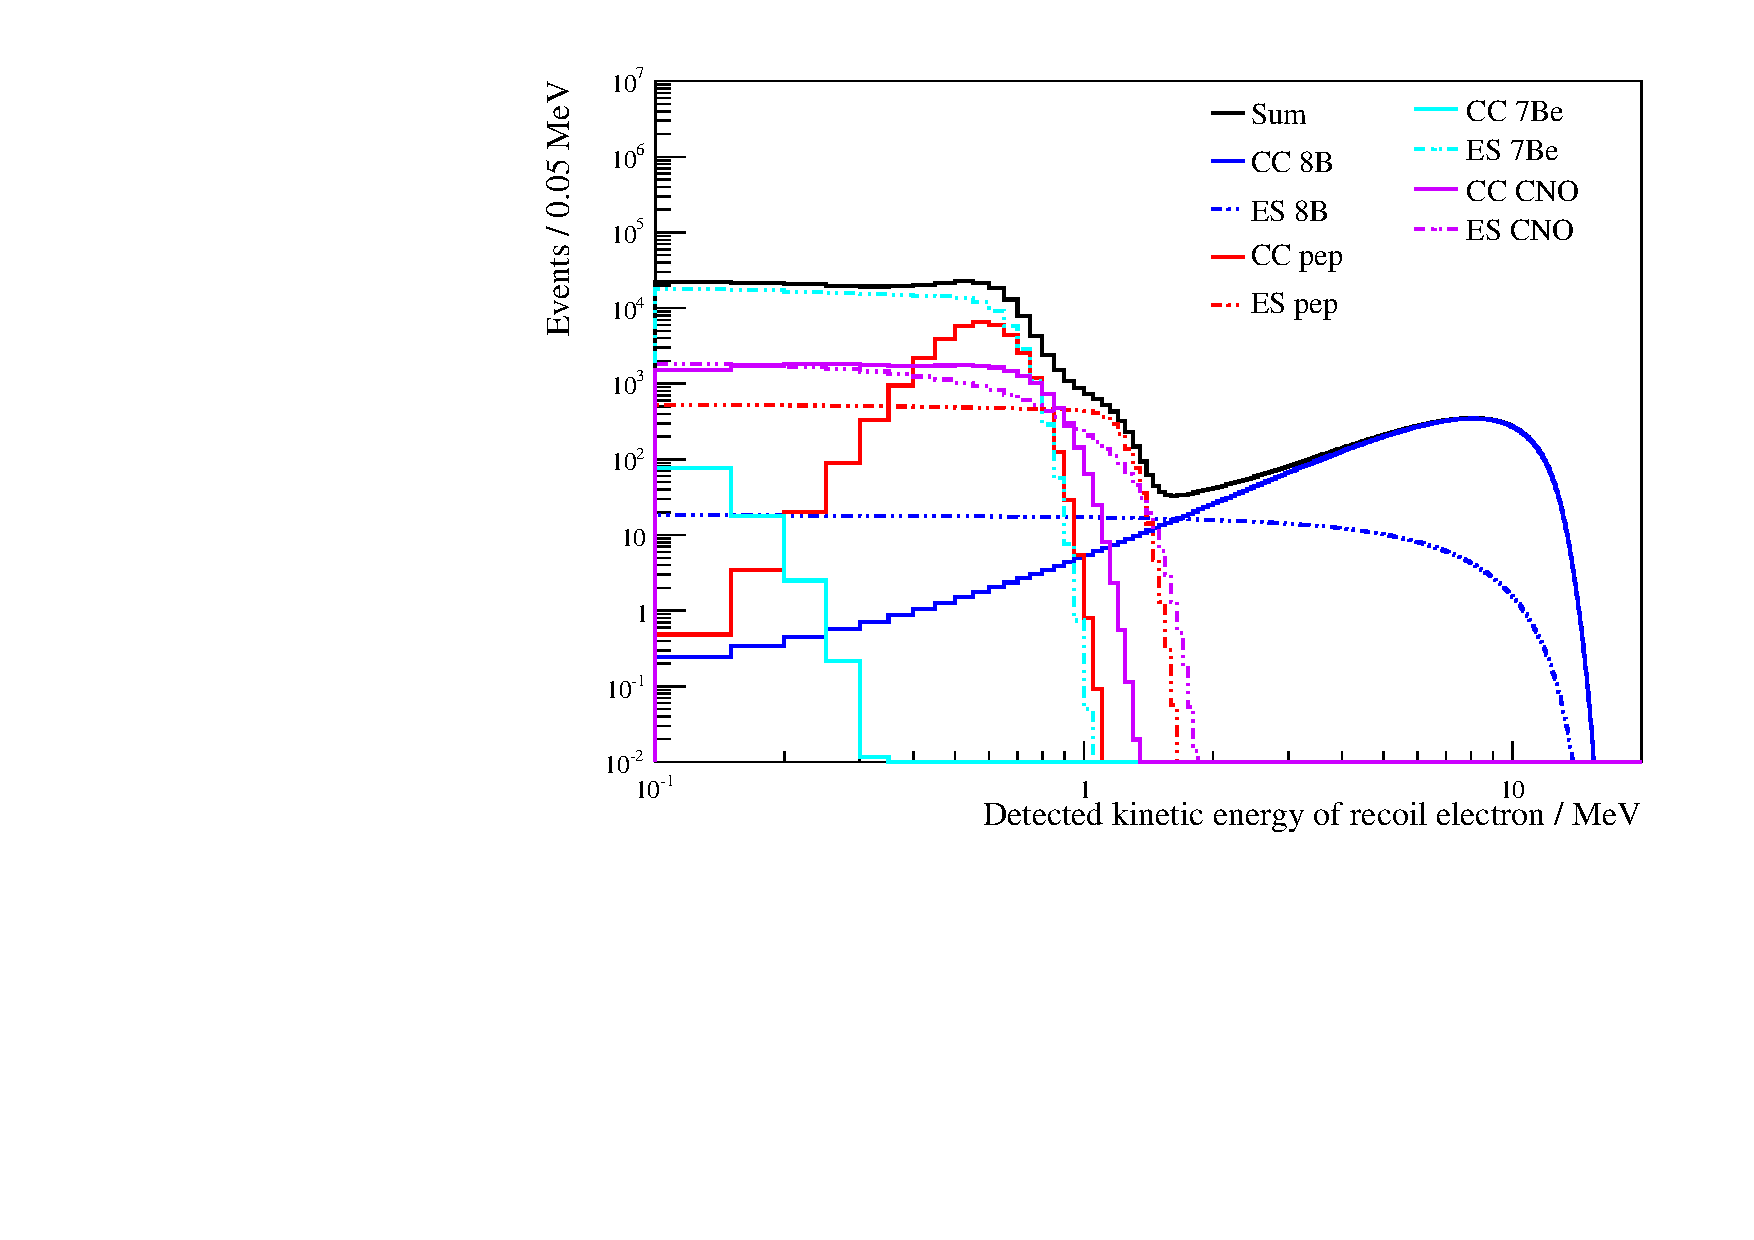
\includegraphics[width=3.5in]{solar/TotalSpectrumCut.pdf}
\caption{(Top) Predicted solar neutrino spectra in a 30-kT WbLS-filled ASDC detector loaded with 1\% $^7$Li by mass.  Light yield of 100 p.e./MeV assumed.  (Bottom) The same spectra with a cut on $\cos\theta_{\odot}=0.4$, reducing the ES component to illustrate the power of CC detection.
\label{f:solarspec}}
\end{center}
\vspace{-1.\baselineskip}
\end{figure}

Due to limited sensitivity, experiments to date have only considered detection of the sum of the three CNO lines.  The increased spectral sensitivity from isotope-loaded WbLS could allow the possibility to separate the constituent lines of the CNO neutrino flux.  The CNO cycle depends critically on temperature in the conversion of C to N, reaching equilibrium only in the most central region of the solar core, where $T > 1.33\times10^7$~K.  In this region, equal numbers of neutrinos are produced in the $\beta^+$ decay of  $^{13}$N and $^{15}$O, whereas in the cooler outer regions only $^{13}$N neutrinos are produced.  Independent measurements of the $^{13}$N and $^{15}$O neutrino fluxes would determine the separate primordial abundances of C and N~\cite{HRS}.  Figure~\ref{f:cno} shows the predicted CNO spectrum broken into its individual components.  A sufficiently sensitive detector with a low enough threshold could separate the contributions from $^{13}$N and $^{15}$O.  A separate measurement of $^{17}$F is unlikely due to the much lower flux; however, there is a strong theoretical basis for fixing the $^{17}$F component to a known fraction of the sum of $^{13}$N  and $^{15}$O.

\begin{figure}[!ht]
\begin{center}
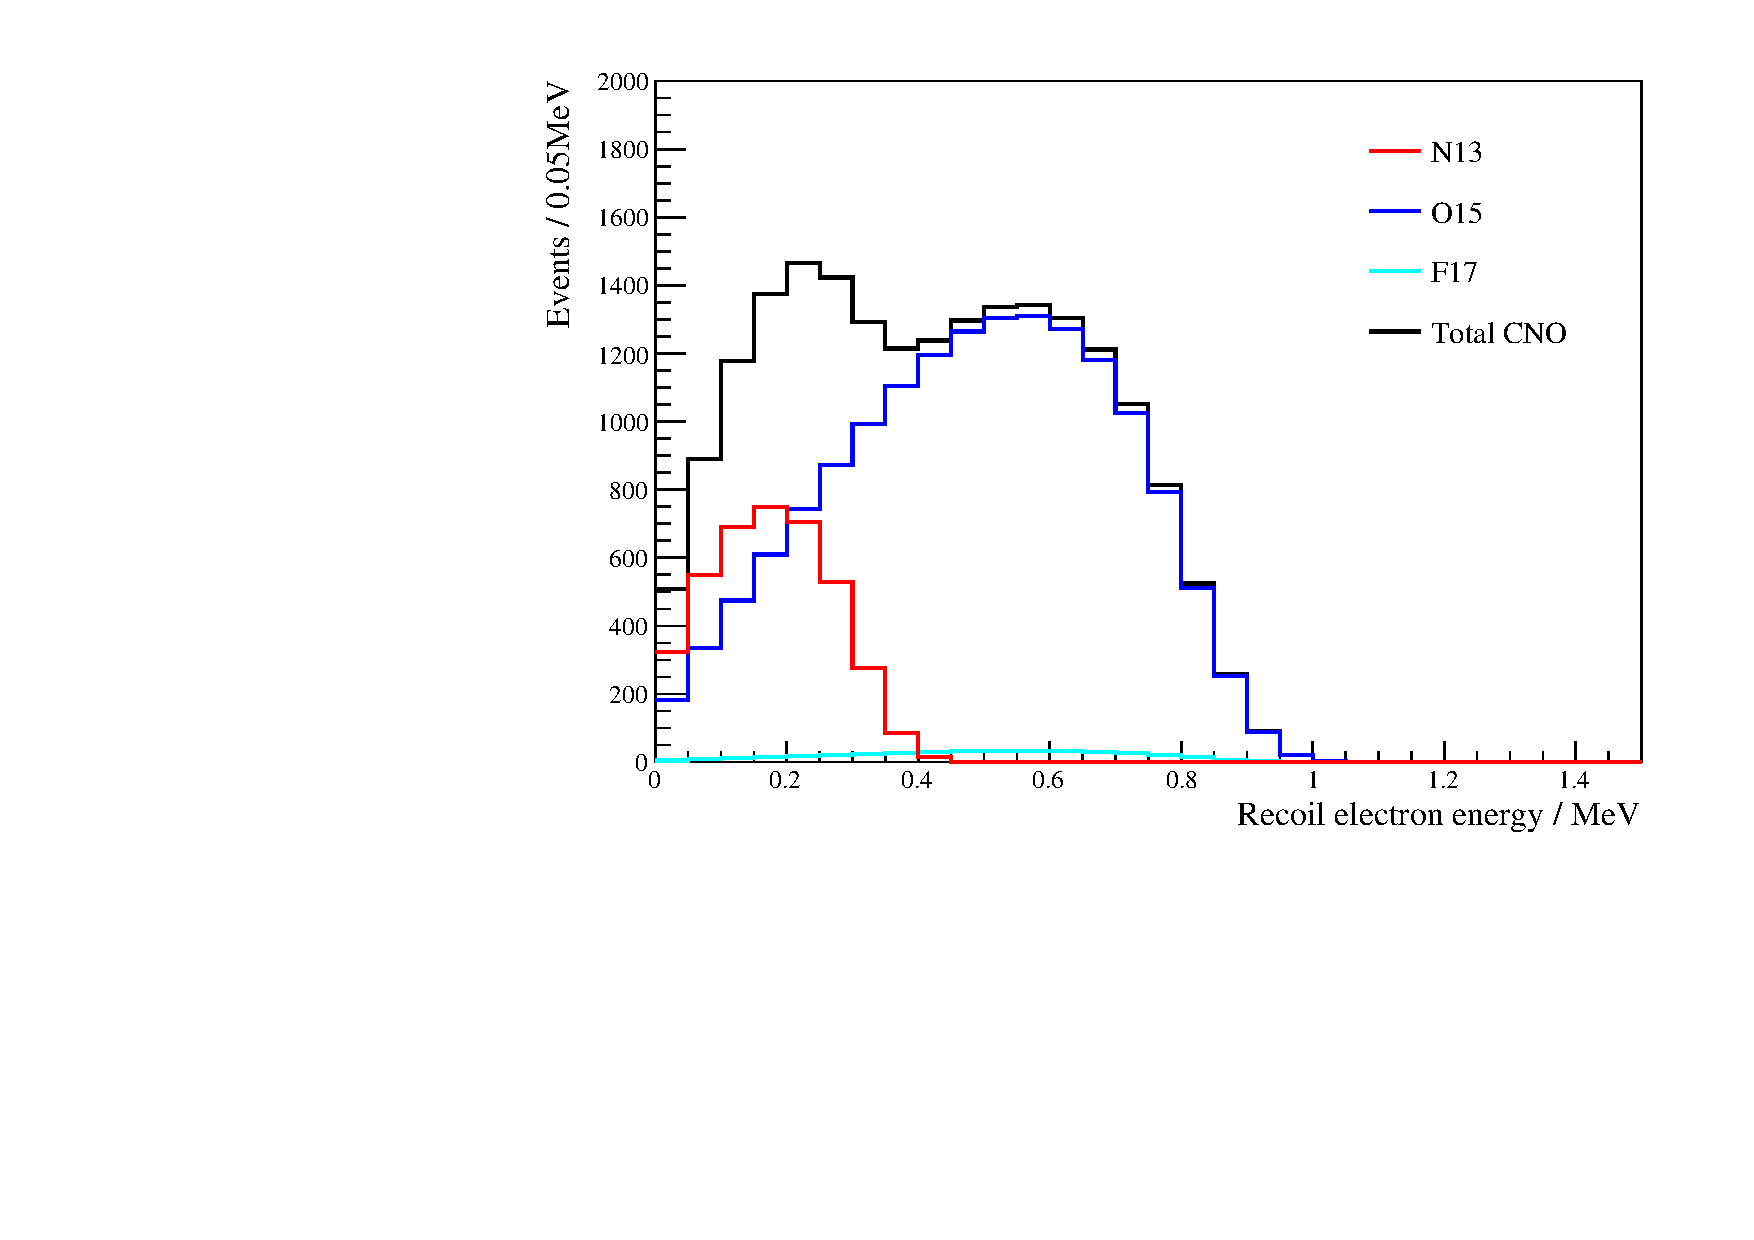
\includegraphics[width=3.5in]{solar/DetectedSpecHistCNO.pdf}
\caption{Predicted spectrum for the individual components of the CNO neutrino flux, and the total, in a WbLS detector.
\label{f:cno}}
\end{center}
\vspace{-1.\baselineskip}
\end{figure}

